\chapter{Error Correction Methods}\label{ch:error_correction}

Since GPS became operational, a range of methodes emerged to improve its positioning accuracy, which were not planned by the inventors of GPS.
These methodes are designed to mitigate the effects of specific errors from section \ref{sec:error_sources}, which can not be modeled.
The remaining errors are:
\begin{itemize}
 \setlength\itemsep{1pt}
 \item satellite modeling errors for ephemeris and clock correction
 \item modeling errors in the ionospheric and tropispheric corrections
 \item the two measurement errors: multipath and receiver noise
\end{itemize}
Three of the most prominent ones are evaluated in this chapter.
They are rated by how effective they are at improving the accuracy and how well they can be implemented on a sounding rocket.


\section{Dual Frequency Measurements}

A relatively new method of error mitigation for civil GPS users are Dual Frequency Measurements.
This only became possible with the launch of Block IIR-M and IIF satellites.
They transmit a second civilian signal on the L2 frequency called L2C.
The benefit of measuring both the L1 C/A and L2C signal is that the ionospheric delay can be determined.
The ionosphere slows down and radio waves, and thus adds a delay to the measured pseudoranges.
This delay depends on the frequency of the radio wave.
With the difference from pseudorange measurement received on different carrier frequencys, the total ionospheric delay can be calculated.

Dual Frequency Measurements can mitigate the ionospheric error, which is one of the biggest error sources, to a large degree.
This error would otherwise have to be modeled with parameter transmitted by the GPS satellites.
The modeled correction only reduces the error by about 50\%.
Used to implement the dual frequency measurements method are a dual frequency receiver and antenna.
\cite{L1_L2}


\section{Carrier-Phase Measurements}

In standard GPS receivers, the C/A-code is tracked to determine the pseudorange.
The C/A-code is sent out with 1023kbit/s, so each chip is about 300m long.
It is modulated onto the sinusoidal L1-carrier with a frequency of 1575.43MHz.
One period of this carrier is only about 19cm long.
This means the carrier would have a much larger resolution than the C/A-code for tracking.
Receiver who use this principle measure the carrier-phase.
The problem with this is the periodical nature of the carrier.
The phase can be measured very precisely, but it can not be directly measured how many whole cycles are between the user and the satellite.
This ambiguity has to be resolved in other ways before the carrier-phase measurement can be used, which can take some time.
After the ambiguity is resolved, the carrier has to be continuously tracked to count the whole cycles.
With the higher resolution, the tracking error introduced by receiver noise can be reduced.

\begin{figure}[ht]
 \centering
 
\includegraphics[height=5cm]{images/Carrier-Phase_Measurement.png}
 \caption{Difference in resolution between C/A-code and L1-carrier}
 \label{fig:carrier_phase}
\end{figure}

Carrier-phase measurements also improve multipath.
The advantage is that reflected signals with a delay of more than a quarter cyrcle do not impact the measurement.
In the case of the L1-carrier, this is only about 5cm.
A typical multipath error for C/A-code measurements is 1-5m.


\section{Differential GPS}

Errors that occure outside of the receiver are correlated for two receivers relatively close together.
The two receivers experience about the same satellite errors and atmospheric delays.
The correlation of those errors depends on the distance between the receivers.
But even with a separation of hundrets of kilometers are the errors still similar.

A receiver at a reference station with a known location can measure the external errors.
If a second receiver (the user) with an unknown location close by corrects its measurements with those measured errors, they cancel out.
This method of error mitigation is called Differential GPS (DGPS).

\begin{figure}[ht]
 \centering
 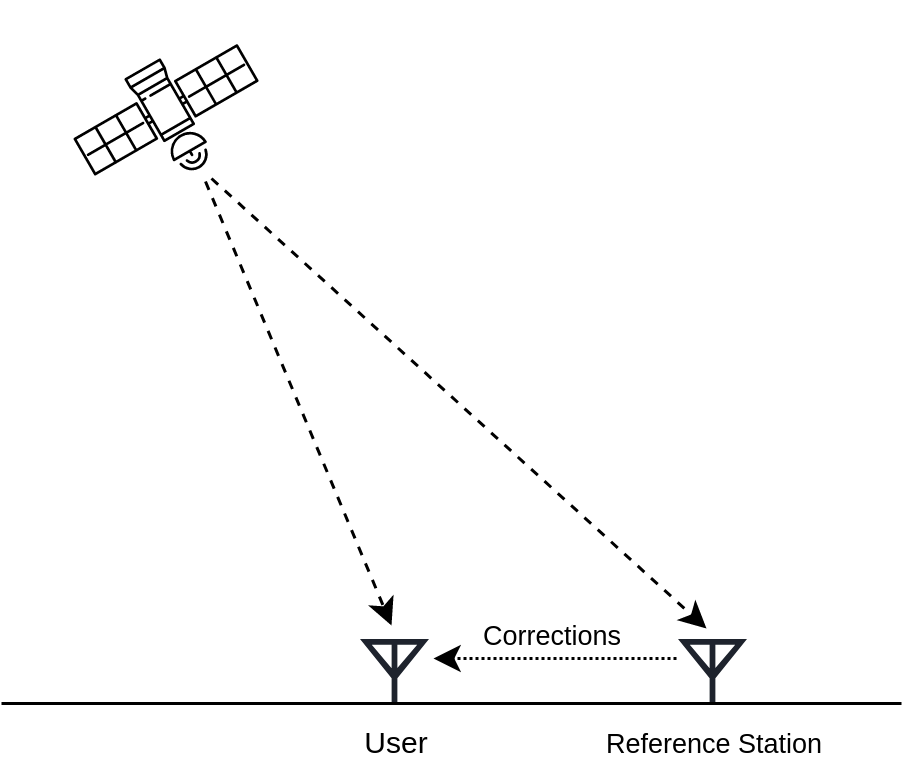
\includegraphics[height=7cm]{images/Differential_GPS.png}
 \caption{Differential GPS concept}
 \label{fig:dgps}
\end{figure}

The easiest way would be to measure the error in the position estimation at the reference station and subtract it in the user position estimation.
The problem with this approach is that it only works if both receivers use the exact same satellites to estimate their position.
This is because the URE of each satellite is correlated between receivers but not necessarily the position estimation.
This is why the reference station does not measure the error in postiton, but the error in the pseudorange of each satellite.
The difference between the actual range and the measured pseudorange is called pseudorange correction (PRC).

A DGPS system generates pseudorange corrections at the reference station and sends them, normally over a wireless link, to the user as shown in figure \ref{fig:dgps}.
The user receiver then corrects its measured pseudoranges with the corrections before it estimates its position.
The benefit of such a system depends on the distance between user and reference station, and the age of the corrections.

Compared to the other methods, DGPS needs a lot of additional infrasturcture.
A reference station and a data link to the user have to be set up.
This is why it is common that the DGPS infrastructure is not maintained by the user, but by a third person that provides this service.
There are also continent-wide systems called Satellite-Based Augmentation Systems (SBAS) like WAAS in the U.S. and EGNOS in Europe.
They transmit the corrections from geostationary satellites directly to the receiver with similar signals as GPS itself.

\section{Summary}

The different methods can mitigate differernt errors.
Dual frequency measurements only mitigate the effect of ionospheric delay.
Carrier-phase measurements and DGPS can reduce the effect of multiple errors.
Carrier-phase measurements the internal ones and DGPS the external.
Combinations of correction methods are also possible like real-time kinematic (RTK).
It is the combination of DGPS with precise carrier-phase measurements.
But with the accuracy rises also the developement effort and the requirements for the infrastructure.